\documentclass[t]{beamer}
\usepackage{mathtools}
\usepackage{tikz}
\usepackage{pgfplots}
\usetikzlibrary{arrows,backgrounds,shapes,matrix,positioning,fit}
\newcommand{\argmax}{\operatornamewithlimits{argmax}}
\newcommand{\argmin}{\operatornamewithlimits{argmin}}
\newcommand{\wt}{\operatornamewithlimits{wt}}
\renewcommand\Re{\operatorname{Re}}
\renewcommand\Im{\operatorname{Im}}

\mode<presentation>
{
  \usetheme{Singapore}
  %\useoutertheme{infolines} % Showing only current section in navigation
  \setbeamertemplate{headline}{}  % Empty headline
  \setbeamertemplate{footline}[frame number]  % Getting rid of footer items except slide number
  \setbeamercovered{invisible}
  \beamertemplatenavigationsymbolsempty % Getting rid of navigation bullets at the bottom
}
\usepackage[english]{babel}
\usepackage[latin1]{inputenc}
\usepackage{times}
\usepackage[T1]{fontenc}

\title[EE 703 DMT]{The Fourier Transform}
\author[Saravanan V]
{
  Saravanan Vijayakumaran\\
  \href{mailto:sarva@ee.iitb.ac.in}{sarva@ee.iitb.ac.in}
}
\institute[IIT Bombay]
{
  Department of Electrical Engineering\\
  Indian Institute of Technology Bombay
}
\date{July 22, 2013}

\AtBeginSection[]%
{%
\begin{frame}[plain]%
  \topskip0pt
  \vspace*{\fill}
    \begin{center}%
      \usebeamerfont{section title}\insertsection%
    \end{center}%
  \vspace*{\fill}
\end{frame}%
}

\begin{document}

%% Frame %%
\begin{frame}
  \titlepage
\end{frame}

%% Frame %%
\begin{frame}{Definition}
  \begin{itemize}
    \item \pause Fourier transform
      \begin{equation*}
        X(f) = \int_{-\infty}^{\infty} x(t) e^{-j2\pi ft} \ dt
      \end{equation*}
    \item \pause Inverse Fourier transform 
      \begin{equation*}
        x(t) = \int_{-\infty}^{\infty} X(f) e^{j2\pi ft} \ df
      \end{equation*}
    \item \pause Notation 
      \begin{equation*}
        x(t) \xrightleftharpoons{} X(f)
      \end{equation*}
  \end{itemize}
\end{frame}

%% Frame %%
\begin{frame}{Properties of Fourier Transform}
  \begin{itemize}
    \item Linearity
      \begin{equation*}
        a x_1(t) + b x_2(t) \xrightleftharpoons{} \pause a X_1(f) + b X_2(f) 
      \end{equation*}
    \pause
    \item Duality
      \begin{equation*}
        X(t) \xrightleftharpoons{} \pause x(-f) 
      \end{equation*}
    \pause
    \item Conjugacy
      \begin{equation*}
        x^{*}(t) \xrightleftharpoons{} \pause X^{*}(-f) 
      \end{equation*}
    \pause
    \item Time scaling
      \begin{equation*}
        x(at) \xrightleftharpoons{} \pause \frac{1}{|a|}X\left(\frac{f}{a}\right)
      \end{equation*}
  \end{itemize}
\end{frame}

%% Frame %%
\begin{frame}{Properties of Fourier Transform}
  \begin{itemize}
    \item Time shift
      \begin{equation*}
        x(t-t_0) \xrightleftharpoons{} \pause e^{-j2\pi ft_0} X(f)
      \end{equation*}
    \pause
    \item Modulation
      \begin{equation*}
        x(t)e^{\ j2\pi f_0t} \xrightleftharpoons{} \pause X(f-f_0)
      \end{equation*}
    \pause
    \item Convolution
      \begin{equation*}
        x(t)\star y(t) \xrightleftharpoons{} \pause X(f)Y(f)
      \end{equation*}
    \pause
    \item Multiplication
      \begin{equation*}
        x(t)y(t) \xrightleftharpoons{} \pause X(f)\star Y(f)
      \end{equation*}
  \end{itemize}
\end{frame}


%% Frame %%
\begin{frame}{Dirac Delta Function}
  \begin{itemize}
    \item \pause Zero for nonzero arguments
      \begin{equation*}
        \delta(t) = 0, \ \ \forall t \neq 0
      \end{equation*}
    \item \pause Unit area
      \begin{equation*}
        \int_{-\infty}^{\infty} \delta(t)\ dt = 1
      \end{equation*}
    \item \pause Sifting property
      \begin{equation*}
        \int_{-\infty}^{\infty}x(t) \delta(t-t_0)\ dt = \pause x(t_0)
      \end{equation*}
    \pause
    \item Fourier transform
      \begin{equation*}
        \delta(t) \xrightleftharpoons{} \pause \int_{-\infty}^{\infty} \delta(t)e^{-j2\pi ft}\ dt = 1
      \end{equation*}
  \end{itemize}
\end{frame}

%% Frame %%
\begin{frame}{Fourier Transforms using Dirac Function}
  \begin{itemize}
    \item DC Signal
      \begin{equation*}
        1 \xrightleftharpoons{} \pause \delta(f)
      \end{equation*}
    \pause
    \item Complex Exponential
      \begin{equation*}
        e^{j2\pi f_ct} \xrightleftharpoons{} \pause \delta(f-f_c)
      \end{equation*}
    \pause
    \item Sinusoidal Functions
      \begin{eqnarray*}
      \cos(2\pi f_c t) & \xrightleftharpoons{} \pause & \frac{1}{2}[\delta(f-f_c) + \delta(f+f_c)]\\
      \pause
      \sin(2\pi f_c t) & \xrightleftharpoons{} \pause & \frac{1}{2j}[\delta(f-f_c) - \delta(f+f_c)]
      \end{eqnarray*}
  \end{itemize}
\end{frame}

%% Frame %%
\begin{frame}{Properties of Fourier Transform}
  \begin{itemize}
    \item Parseval's theorem
      \begin{equation*}
        \int_{-\infty}^{\infty} x(t)y^*(t) \ dt = \pause \int_{-\infty}^{\infty} X(f)Y^*(f)\ df
      \end{equation*}
    \pause
    \item Rayleigh's theorem
      \begin{equation*}
        \int_{-\infty}^{\infty} |x(t)|^2\ dt = \pause \int_{-\infty}^{\infty} |X(f)|^2\ df
      \end{equation*}
  \end{itemize}
\end{frame}

%% Frame %%
\begin{frame}{Signum Function}
  \begin{columns}
    \begin{column}{0.5\textwidth}
      \begin{equation*}
        \text{sgn}(t) = \left\{
                  \begin{array}{rr}
                  +1, & t > 0 \\
                   0, & t = 0 \\
                  -1, & t < 0 
                  \end{array}
                \right.
      \end{equation*}
    \end{column}

    \begin{column}{0.5\textwidth}
      \begin{figure}
        \centering
          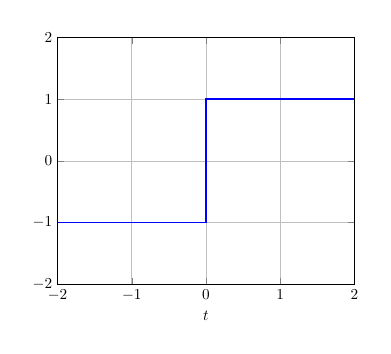
\begin{tikzpicture}[scale=0.55,transform shape]
            \begin{axis}[xlabel=$t$,xmax=2,xmin=-2,ymax=2,ymin=-2,grid=major]
              \addplot[color=blue,very thick] coordinates {(-2,-1) (0,-1) (0,1) (2,1)};
            \end{axis}
          \end{tikzpicture}
      \end{figure}
    \end{column}
  \end{columns}
  \pause
  Fourier Transform
  \begin{equation*}
    \text{sgn}(t) \xrightleftharpoons{} \pause \frac{1}{j\pi f}
  \end{equation*}

\end{frame}

%% Frame %%
\begin{frame}{Signum Function}
  \begin{columns}
    \begin{column}{0.5\textwidth}
      \begin{equation*}
        g(t) = \left\{
                  \begin{array}{rr}
                  e^{-at}, & t > 0 \\
                   0, & t = 0 \\
                  -e^{at}, & t < 0 
                  \end{array}
                \right.
      \end{equation*}
    \end{column}

    \begin{column}{0.5\textwidth}
      \begin{figure}
        \centering
          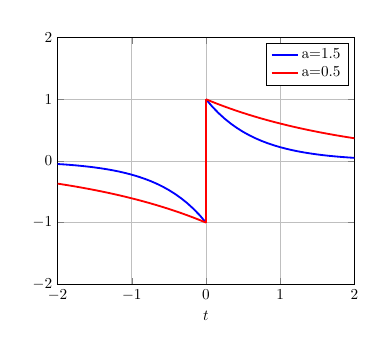
\begin{tikzpicture}[scale=0.55,transform shape]
            \begin{axis}[xlabel=$t$,xmax=2,xmin=-2,ymax=2,ymin=-2,grid=major]
              \addplot[color=blue,very thick,domain=0:2,forget plot] {exp(-1.5*x)};
              \addplot[color=blue,very thick,domain=-2:0,forget plot] {-exp(1.5*x)};
              \addplot[color=blue,very thick] coordinates {(0,-1) (0,1)};
              \addlegendentry{a=1.5}
              \addplot[color=red,very thick,domain=0:2,forget plot] {exp(-0.5*x)};
              \addplot[color=red,very thick,domain=-2:0,forget plot] {-exp(0.5*x)};
              \addplot[color=red,very thick] coordinates {(0,-1) (0,1)};
              \addlegendentry{a=0.5}
            \end{axis}
          \end{tikzpicture}
      \end{figure}
    \end{column}
  \end{columns}
  \pause
  \begin{equation*}
    \text{sgn}(t) = \lim_{a \rightarrow 0^+} g(t)
  \end{equation*}
  \pause
  \begin{equation*}
    G(f) = \frac{-j4\pi f}{a^2+(2\pi f)^2}
  \end{equation*}
\end{frame}

%% Frame %%
\begin{frame}{Unit Step Function}
  \begin{columns}
    \begin{column}{0.5\textwidth}
      \begin{equation*}
          u(t) = \left\{
                  \begin{array}{rr}
                  1, & t > 0 \\
                  \frac{1}{2}, & t = 0 \\
                  0, & t < 0 
                  \end{array}
                \right.
      \end{equation*}
    \end{column}

    \begin{column}{0.5\textwidth}
      \begin{figure}
        \centering
          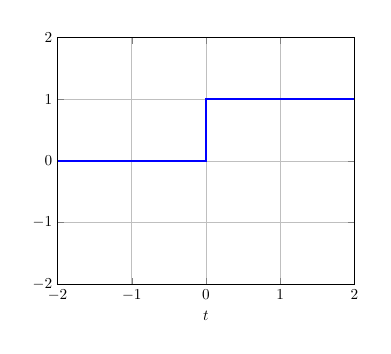
\begin{tikzpicture}[scale=0.55,transform shape]
            \begin{axis}[xlabel=$t$,xmax=2,xmin=-2,ymax=2,ymin=-2,grid=major]
              \addplot[color=blue,very thick] coordinates {(-2,0) (0,0) (0,1) (2,1)};
            \end{axis}
          \end{tikzpicture}
      \end{figure}
    \end{column}
  \end{columns}
  \pause
  Fourier Transform
  \begin{equation*}
    u(t) \xrightleftharpoons{} \pause \frac{1}{j2\pi f} + \frac{1}{2}\delta(f)
  \end{equation*}
  \pause
  \begin{equation*}
    u(t) = \frac{1}{2}[\text{sgn}(t) + 1]
  \end{equation*}
\end{frame}

%% Frame %%
\begin{frame}{Properties of Fourier Transform}
  \begin{itemize}
    \item Differentiation
      \begin{equation*}
        \frac{d}{dt} x(t) \xrightleftharpoons{} \pause j2\pi f\  X(f)
      \end{equation*}
    \pause
    \item Integration
      \begin{equation*}
        \int_{-\infty}^{t} x(\tau) \ d\tau \xrightleftharpoons{} \pause \frac{X(f)}{j2\pi f} + \frac{1}{2} X(0)\delta(f)
      \end{equation*}
  \end{itemize}
\end{frame}

%% Frame %%
\begin{frame}{Rectangular Pulse}
  \begin{columns}
    \begin{column}{0.4\textwidth}
      \begin{equation*}
          \Pi(t) = \left\{
                  \begin{array}{rr}
                  1, & |t| \leq \frac{1}{2} \\
                  0, & |t| > \frac{1}{2} 
                  \end{array}
                \right.
      \end{equation*}
    \end{column}

    \begin{column}{0.6\textwidth}
      \begin{figure}
        \centering
          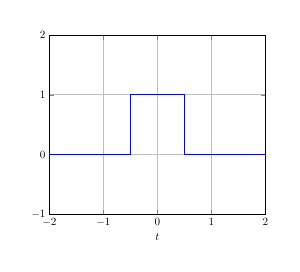
\begin{tikzpicture}[scale=0.40,transform shape]
            \begin{axis}[xlabel=$t$,xmax=2,xmin=-2,ymax=2,ymin=-1,grid=major]
              \addplot[color=blue,very thick,domain=-2:2] coordinates {(-2,0) (-0.5,0) (-0.5,1) (0.5,1) (0.5,0) (2,0)};
            \end{axis}
          \end{tikzpicture}
      \end{figure}
    \end{column}
  \end{columns}
  \pause
  Fourier Transform

\begin{columns}
	\begin{column}{0.4\textwidth}
  \begin{equation*}
    \Pi\left(\frac{t}{T}\right) \xrightleftharpoons{} \pause T\text{sinc}(fT)
  \end{equation*}
	\end{column}

	\begin{column}{0.6\textwidth}
      \begin{figure}
        \centering
          \begin{tikzpicture}[scale=0.40,transform shape]
            \begin{axis}[xlabel=$f$,xmax=5,xmin=-5,ymax=2,ymin=-1,grid=major]
              \addplot[color=blue,very thick,domain=-5:5,samples=1000] gnuplot{sin(pi*x)/(pi*x)};
            \end{axis}
          \end{tikzpicture}
      \end{figure}
	\end{column}
\end{columns}
\end{frame}


\begin{frame}{}
\vfill
\begin{center}
Thanks for your attention
\end{center}
\vfill
\end{frame}

\end{document}
